\chapter{Iteration 1: Design and Implementation}
\label{chap:iter1}
\textbf{Baseline.} This chapter describes the code as it stood at the mid-report
tag \texttt{v0.2.0-mid2} (\texttt{678acbd}, 13~October 2026). Work after that
date is Iteration~2 and is described in Chapter~\ref{chap:iter2}.

\section{Iteration Objectives}
Iteration 1 targeted the spatio-temporal memory engine (FR3), with light work on
FR1 and FR2. It covered geometry, object detection and 3D lifting, semantic
anchors, instance association, events and an item query. It did not establish
a live-to-memory path.

\section{Selected Use Cases / Features}
The selected use cases were UC-01 (capture and ingest) and UC-03 (find the last
known location of an object). The slice also supports a partial UC-04 timeline
view.

\section{Design}
Figures~\ref{fig:i1-core}--\ref{fig:i1-api} are class diagrams drawn from the
code at \texttt{v0.2.0-mid2}.

\aegisfig{ch6-class-core-models}
  {Iteration 1 core models: configuration, vocabulary, frames, poses and 3D boxes.}
  {fig:i1-core}
\aegisfig{ch6-class-scene-graph-v1}
  {Iteration 1 scene graph (schema 1): anchors, object instances, per-frame
   timeline and events.}
  {fig:i1-graph}
\aegisfig{ch6-class-live}
  {Iteration 1 live MJPEG sampler (not yet joined to the pipeline).}
  {fig:i1-live}
\aegisfig{ch6-class-api}
  {Iteration 1 API and \texttt{QueryReasoningEngine}.}
  {fig:i1-api}
\aegisfig{batchvideosamplingflowchart}
  {Batch video sampling and reconstruction keyframe selection.}
  {fig:algorithm-flow}

\section{Implementation}
The Python package uses a \texttt{src} layout. \path{ingestion/video.py}
samples a video and writes frames and metadata; \path{geometry/vggt_runner.py}
writes pointmaps, confidence maps, point clouds and poses;
\path{perception/} detects objects with YOLOE (open-vocabulary prompts),
refines masks with SAM~2 and lifts them to 3D boxes; \path{memory/anchors.py}
clusters furniture into anchors; \path{memory/association.py} keeps object
identities across frames with a radius and an HSV appearance check;
\path{memory/scene_graph.py} writes the schema-1 graph with a per-frame
timeline; \path{memory/reasoning.py} answers ``where is X'' from the latest
observation; \path{remote/api.py} serves the graph, queries and timelines.
The Flutter client \path{apps/mobile} showed answers and evidence.

\section{Completed Features}
Iteration~1 delivered the batch artifact pipeline on Modal, the schema-1 memory,
the item-query API with a latency assertion on fixtures, the CI pipeline
(\texttt{v0.1.0-mid1}, 4~October), the in-hand memory and Rerun view, the
stand-alone live MJPEG sampler and a redesigned Flutter UI with search history
(\texttt{v0.2.0-mid2}). Compaction, speech, authenticated caregiver access and
the live-to-memory link were not part of Iteration~1.

\section{Technical Implementation Details}
VGGT keyframe stride was 6. Anchor extraction used a 0.40 geometric-unit cluster
threshold. Coordinates were displayed through a fixed \texttt{SCALE = 5.0} and a
\texttt{to\_zup} axis swap, which Iteration~2 removed (AD1). Geometric values
are VGGT units, not calibrated metres.

\section{Tools, Frameworks and Technologies}
Python 3.12, uv, OpenCV, NumPy, FastAPI, Uvicorn, Modal, VGGT-$\Omega$,
YOLOE/YOLO-World (Ultralytics), SAM~2, Rerun, Flutter/Dart and GitHub Actions.
Modal provides CPU workers for preprocessing and Rerun and L4 GPU workers for
VGGT and perception, with data at \path{/data} and the model cache at
\path{/models}.

\section{Demonstration Evidence}
\begin{figure}[H]\centering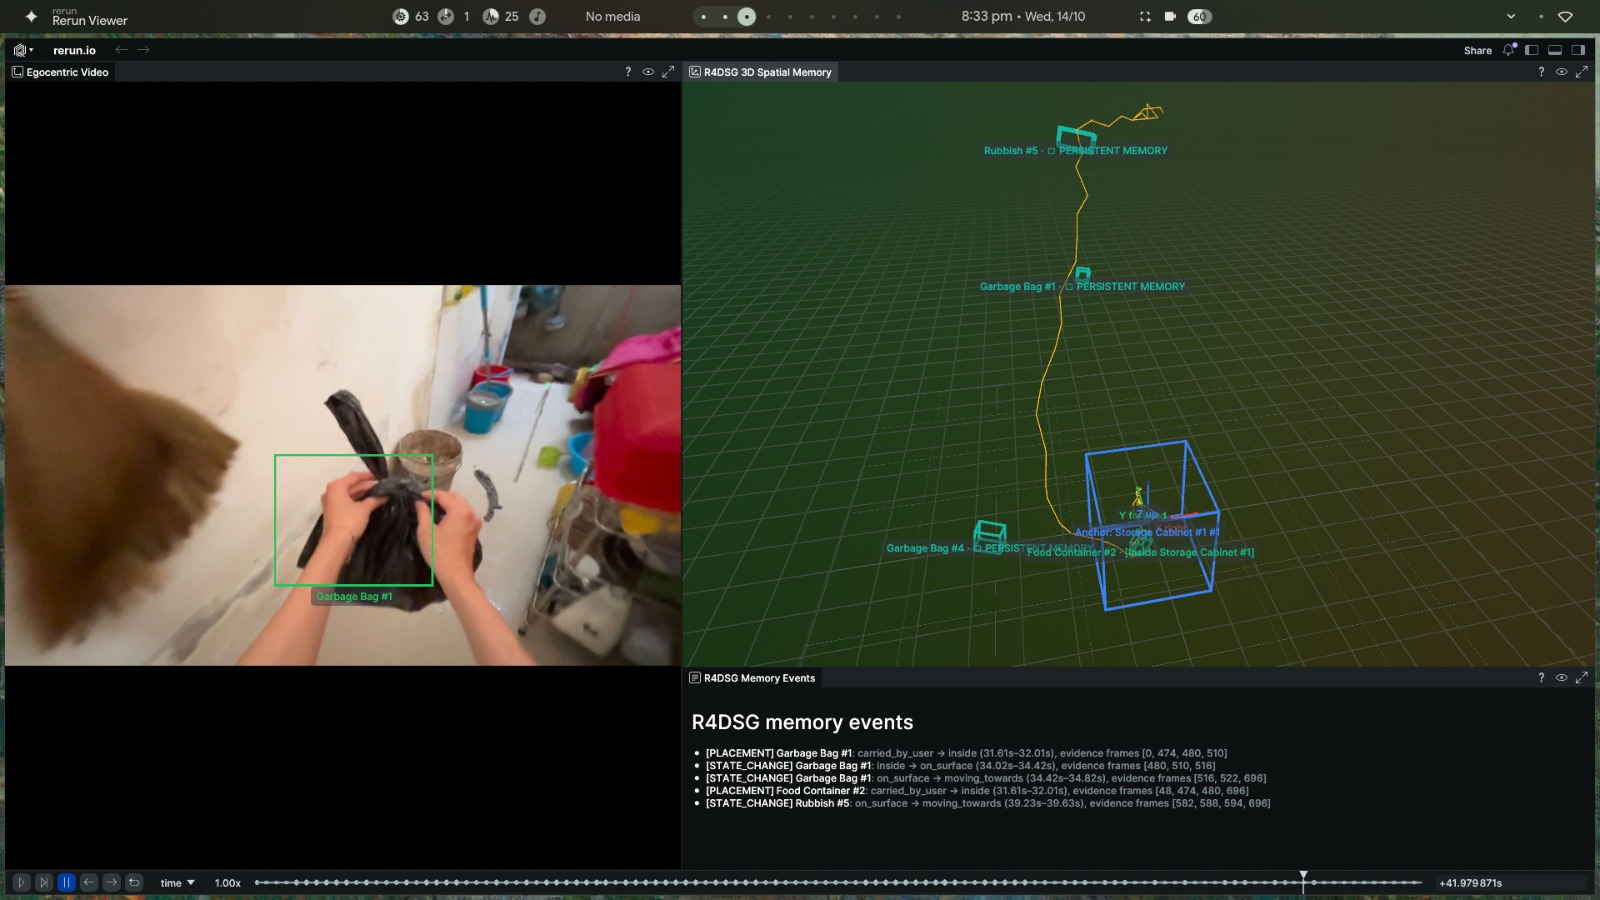
\includegraphics[width=\textwidth,height=0.55\textheight,keepaspectratio]{ThesisFigs/chapter6-screenshot-evidence.jpeg}\caption{Iteration~1 prototype screenshot (mid report).}\label{fig:screenshot-evidence}\end{figure}

\section{Iteration Outcome}
\label{sec:iter1-outcome}
The Iteration~1 artifact, API and client slice was implemented and tested in CI.
Its exit criteria were only partly evidenced: AC-06 (restart equivalence) and the
item query passed on fixtures, but no live capture reached memory, YOLOE missed
most small personal objects (it was replaced by SAM~3 in Iteration~2,
Section~\ref{sec:experiments}), and the per-frame timeline made the graph grow
with video length. These three findings set the Iteration~2 scope.
